\documentclass[11pt,a4paper]{article}

\usepackage{fontspec}
\usepackage[french]{babel}
\usepackage{amsmath}
\usepackage[margin=2.5cm]{geometry}
\usepackage{graphicx}
\usepackage{booktabs}
\usepackage{array}
\usepackage{longtable}
\usepackage{float}
\usepackage{caption}
\usepackage{setspace}
\usepackage{xurl}
\usepackage[hidelinks,hypertexnames=false]{hyperref}

\graphicspath{{figures/}}
\setstretch{1.15}
\setlength{\parskip}{0.4em}
\captionsetup{font=small}

\begin{document}

% ------------------------------------------------------------------
% Page de titre
% ------------------------------------------------------------------
\begin{titlepage}
\centering
\vspace*{2cm}
{\large Séminaire BI et Data Viz\par}
\vspace{0.3cm}
{\large Enseignant : Ismail Rebai\par}
\vspace{3cm}
{\LARGE\bfseries Que contient l'eau de votre robinet ?\par}
\vspace{0.6cm}
{\Large Qualité de l'eau potable en France de 2021 à 2026\par}
\vspace{0.3cm}
{\large Rapport de projet\par}
\vspace{3cm}
{\large Réalisé par :\par}
\vspace{0.3cm}
Mohammed BENAKKA OUAYAD\par
Hajar BITARI\par
Aya SINDEL\par
\vfill
{\large Novembre 2026\par}
\end{titlepage}

\tableofcontents
\newpage

% ------------------------------------------------------------------
\section{Introduction}
% ------------------------------------------------------------------

L'eau du robinet est souvent présentée comme l'aliment le plus contrôlé en France. Chaque année, les Agences régionales de santé (ARS) réalisent plusieurs centaines de milliers de prélèvements sur les réseaux de distribution et y mesurent des dizaines de paramètres. Malgré ce suivi, la qualité de l'eau revient régulièrement dans l'actualité, en particulier à cause des résidus de pesticides et, plus récemment, des PFAS, appelés « polluants éternels ».

Les résultats de ces contrôles sont publics, mais ils sont publiés sous forme de fichiers très volumineux qui ne sont pas exploitables directement par un décideur ou par un citoyen. L'objectif de notre projet est de transformer ces données en tableaux de bord clairs, réalisés avec Tableau, pour aider à répondre à une question concrète : où faut-il agir en priorité ?

Ce rapport présente successivement le contexte et la problématique, les données utilisées et leur préparation, la méthode retenue, la réalisation du classeur Tableau, les résultats obtenus, puis les recommandations et les limites de notre travail.

% ------------------------------------------------------------------
\section{Contexte et problématique}
% ------------------------------------------------------------------

\subsection{Contexte}

L'eau distribuée au robinet fait l'objet d'un contrôle sanitaire organisé par les ARS. Les prélèvements sont analysés par des laboratoires agréés et les résultats sont enregistrés dans la base nationale SISE-Eaux du ministère de la Santé. Pour chaque paramètre réglementé, une limite de qualité fixe la valeur à ne pas dépasser.

Plusieurs sujets rendent cette question actuelle. Les pesticides et surtout leurs produits de dégradation (les métabolites) sont détectés dans de nombreux captages. Les PFAS, des substances chimiques très persistantes, font l'objet d'une nouvelle limite européenne, applicable depuis le 1\textsuperscript{er} janvier 2026. Enfin, les nitrates et les contaminations bactériennes restent des problèmes connus dans certains territoires.

\subsection{Problématique}

Nous avons formulé la problématique suivante :

\begin{quote}
\textit{Où l'eau du robinet dépasse-t-elle les limites sanitaires en France, et quels départements une Agence régionale de santé doit-elle traiter en priorité ?}
\end{quote}

Autrement dit, si une ARS dispose d'un budget limité, où doit-elle intervenir en premier ? Pour y répondre, nous avons cherché à savoir quels polluants dépassent le plus souvent les limites, quels territoires sont les plus touchés, comment la situation évolue depuis 2021 et combien d'habitants sont concernés.

\subsection{Les utilisateurs visés}

Nous avons pensé le projet pour deux types d'utilisateurs. Le premier est le décideur public (ARS, préfecture ou ministère), qui a besoin d'une vue d'ensemble pour comparer les territoires et fixer des priorités. Le second est le citoyen, qui veut simplement savoir si l'eau de sa commune pose problème. Chacun dispose de son propre tableau de bord : « Vue France » pour le décideur et « Ma commune » pour le citoyen.

% ------------------------------------------------------------------
\section{Les données}
% ------------------------------------------------------------------

\subsection{Source}

Les données proviennent du jeu « Résultats du contrôle sanitaire de l'eau distribuée commune par commune », publié par le ministère de la Santé sur data.gouv.fr sous Licence Ouverte. Nous avons utilisé les fichiers des années 2021 à 2026. L'année 2026 est incomplète : elle couvre les prélèvements de janvier à septembre. Pour placer les communes sur une carte et connaître leur population, nous avons ajouté le référentiel des communes de l'Insee (via l'API geo.api.gouv.fr).

Chaque année est livrée sous forme d'une archive d'environ 230 à 310~Mo, soit 1,7~Go compressés pour les six années et plus de 11~Go une fois décompressés.

\subsection{Structure des fichiers bruts}

Chaque archive annuelle contient trois tables :

\begin{itemize}
  \item la table \textbf{communes et réseaux}, qui indique quelle unité de distribution (réseau) alimente quelle commune ;
  \item la table des \textbf{prélèvements}, avec la date, le lieu, le réseau et la conclusion de conformité de chaque échantillon (environ 290~000 par an) ;
  \item la table des \textbf{résultats d'analyses}, avec pour chaque prélèvement le paramètre mesuré, la valeur obtenue et la limite de qualité (environ 13 millions de lignes par an de 2021 à 2025).
\end{itemize}

Les prélèvements sont reliés aux résultats par le code du prélèvement, et aux communes par le code du réseau. Au total, nous avons traité 1~635~605 prélèvements sur la période.

\subsection{Les cinq familles de polluants}

Pour rendre l'analyse lisible, nous avons regroupé les paramètres soumis à une limite sanitaire en cinq familles (tableau~\ref{tab:familles}).

\begin{table}[H]
\centering
\small
\begin{tabular}{>{\raggedright}p{2.6cm} >{\raggedright}p{4.6cm} >{\raggedright\arraybackslash}p{6.6cm}}
\toprule
Famille & Exemples & Enjeu \\
\midrule
Bactéries & \textit{Escherichia coli}, entérocoques & Risque immédiat (gastro-entérites), signe d'une contamination fécale \\
Nitrates & Nitrates (limite 50~mg/L), nitrites & Origine agricole, risque surtout pour les nourrissons et les femmes enceintes \\
Pesticides & Chloridazone desphényl, chlorothalonil R417888, atrazine déséthyl & Résidus agricoles et métabolites, exposition chronique \\
PFAS & Somme de 20 PFAS (limite 0,1~µg/L) & Substances très persistantes, nouvelle limite européenne en 2026 \\
Autres substances & Turbidité, chlorure de vinyle, métaux & Paramètres physico-chimiques divers \\
\bottomrule
\end{tabular}
\caption{Les cinq familles de polluants retenues}
\label{tab:familles}
\end{table}

\subsection{Vocabulaire utilisé}

Dans la suite du rapport, un \textit{prélèvement} désigne un échantillon d'eau prélevé en un point du réseau, et une \textit{analyse} la mesure d'un paramètre dans ce prélèvement. On parle de \textit{dépassement} lorsqu'une valeur mesurée est supérieure à sa limite de qualité. Une \textit{commune touchée} est une commune qui a connu au moins un dépassement dans l'année pour une famille donnée, et la \textit{population exposée} est la population de ces communes.

% ------------------------------------------------------------------
\section{Préparation des données}
% ------------------------------------------------------------------

\subsection{Étapes de traitement}

Les fichiers bruts étaient beaucoup trop lourds pour être chargés tels quels dans Tableau Public. Nous les avons donc préparés en amont, en suivant les étapes suivantes :

\begin{enumerate}
  \item téléchargement des six archives annuelles depuis data.gouv.fr ;
  \item nettoyage : codes de communes et de départements conservés sous forme de texte (pour garder le « 01 » ou le « 2A »), harmonisation des dates, suppression des doublons ;
  \item classement de chaque paramètre dans l'une des cinq familles ;
  \item comparaison de chaque résultat à sa limite de qualité pour repérer les dépassements ;
  \item agrégation à plusieurs niveaux (commune, département, mois, substance) et calcul du score de priorité ;
  \item ajout de la latitude et de la longitude des communes et des départements pour les cartes.
\end{enumerate}

Un point a demandé une attention particulière : un même prélèvement peut être rattaché à plusieurs réseaux de distribution. Sans précaution, il aurait été compté plusieurs fois. Nous avons donc compté les prélèvements de manière distincte : par commune pour les fichiers communaux, et par département gestionnaire pour la synthèse départementale, où chaque prélèvement n'est compté qu'une seule fois. De la même façon, lorsqu'un paramètre était mesuré deux fois sur un même prélèvement (sur le terrain et en laboratoire), nous avons gardé la valeur la plus défavorable.

\subsection{Fichiers produits}

Le traitement aboutit à six fichiers CSV (tableau~\ref{tab:fichiers}). Chacun décrit la même réalité à un niveau de détail différent, ce qui évite de faire des jointures dans Tableau : chaque feuille du classeur utilise une seule source.

\begin{table}[H]
\centering
\small
\begin{tabular}{>{\raggedright}p{5.4cm} >{\raggedright}p{3.8cm} >{\raggedright\arraybackslash}p{4.8cm}}
\toprule
Fichier & Une ligne correspond à & Utilisation \\
\midrule
1\_communes\_qualite\_eau & commune, famille et année & archive, non utilisé dans le classeur \\
1b\_communes\_2025\_leger & commune et famille (2025) & carte des communes, fiche commune, population exposée \\
2\_departements\_synthese & département, famille et année & évolution par famille, carte de chaleur \\
3\_prelevements\_conformite & département et mois & évolution de la conformité, chiffres clés \\
4\_substances & substance et année & classement des substances \\
5\_score\_priorite\_departements & département et année & carte des départements, Top 10 \\
\bottomrule
\end{tabular}
\caption{Les six fichiers préparés pour Tableau}
\label{tab:fichiers}
\end{table}

% ------------------------------------------------------------------
\section{Analyse descriptive}
% ------------------------------------------------------------------

Avant de construire les visualisations, nous avons décrit les données. Le nombre de prélèvements est stable, autour de 290~000 par an (tableau~\ref{tab:volumes}). En 2025, 295~134 prélèvements ont été réalisés et 34~807 communes ont été contrôlées, soit la quasi-totalité des communes françaises.

\begin{table}[H]
\centering
\small
\begin{tabular}{lrrr}
\toprule
Année & Prélèvements & Non conformes & Taux de non-conformité \\
\midrule
2021 & 286~231 & 15~594 & 5,45~\% \\
2022 & 290~091 & 16~121 & 5,56~\% \\
2023 & 292~739 & 16~451 & 5,62~\% \\
2024 & 291~616 & 16~835 & 5,77~\% \\
2025 & 295~134 & 13~296 & 4,51~\% \\
2026 (janvier à septembre) & 179~794 & 8~173 & 4,55~\% \\
\bottomrule
\end{tabular}
\caption{Volume de prélèvements et non-conformité par année}
\label{tab:volumes}
\end{table}

Cette analyse a fait apparaître un point important pour la suite : les PFAS n'étaient presque pas mesurés avant 2025. Le nombre de communes où ils ont été recherchés passe de 227 en 2022 à 27~865 en 2025 (figure~\ref{fig:pfas}). Toute comparaison des PFAS dans le temps serait donc trompeuse, et nous les avons exclus des courbes d'évolution.

\begin{figure}[H]
\centering
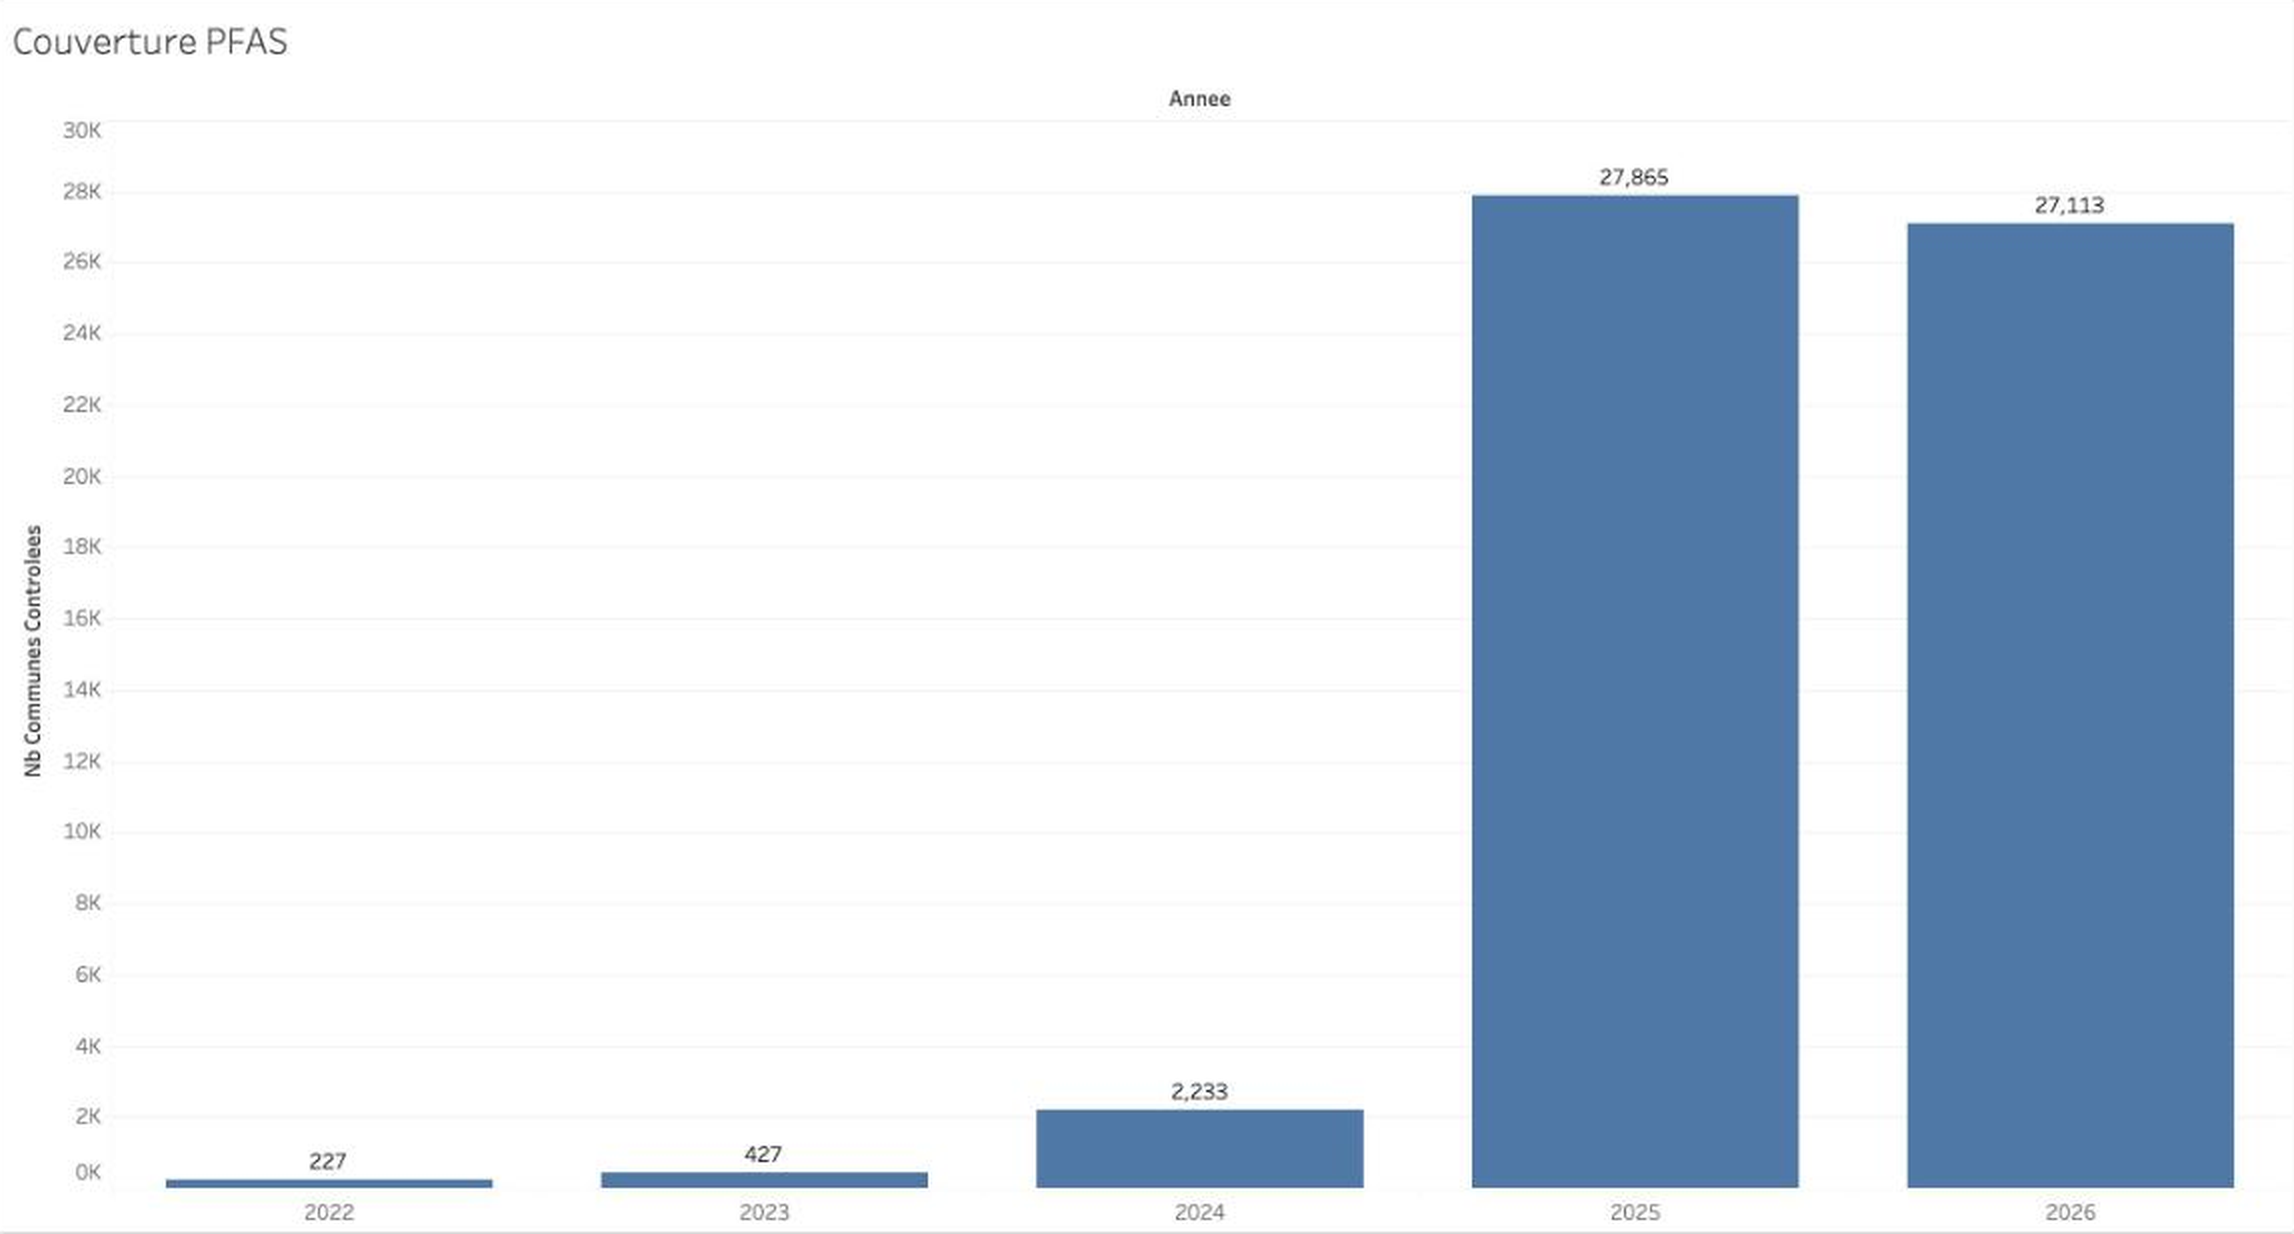
\includegraphics[width=0.75\textwidth]{couverture_pfas.png}
\caption{Nombre de communes où les PFAS ont été mesurés (2026 : janvier à septembre)}
\label{fig:pfas}
\end{figure}

% ------------------------------------------------------------------
\section{Méthode}
% ------------------------------------------------------------------

\subsection{Des taux plutôt que des comptes}

Un département très peuplé compte forcément plus de prélèvements, donc plus de dépassements, qu'un département rural. Comparer des nombres bruts n'aurait donc pas de sens. Nous avons travaillé avec des taux :

\[
\text{Taux de dépassement} = \frac{\text{prélèvements avec au moins un dépassement}}{\text{prélèvements analysés}}
\]

Pour la conformité globale, nous avons utilisé l'indicateur officiel de conformité de chaque prélèvement, qui tient compte de l'ensemble des paramètres.

\subsection{Le score de priorité}

Pour classer les départements, nous avons construit un score de priorité. Pour chaque famille, le risque d'un département est la part de sa population concernée, pondérée par le taux de dépassement observé dans chaque commune. Le score est ensuite une moyenne pondérée de ces cinq risques :

\[
\text{score} = 0{,}30 \times \text{bactéries} + 0{,}20 \times \text{nitrates} + 0{,}20 \times \text{pesticides} + 0{,}20 \times \text{PFAS} + 0{,}10 \times \text{autres}
\]

\begin{table}[H]
\centering
\small
\begin{tabular}{l c >{\raggedright\arraybackslash}p{8.5cm}}
\toprule
Famille & Poids & Justification \\
\midrule
Bactéries & 30~\% & Seul risque immédiat pour la santé, qui demande une action rapide \\
Nitrates & 20~\% & Risque chronique, surtout pour les nourrissons \\
Pesticides & 20~\% & Exposition chronique \\
PFAS & 20~\% & Substances très persistantes \\
Autres substances & 10~\% & Famille très hétérogène, de la turbidité à des métaux comme le plomb ; poids plus faible par choix \\
\bottomrule
\end{tabular}
\caption{Poids retenus pour le score de priorité}
\label{tab:poids}
\end{table}

Ces poids sont un choix de décideur et non une vérité scientifique. Une amélioration possible serait d'ajouter dans Tableau un paramètre pour les modifier et voir le classement évoluer. Le rang 1 correspond au département le plus prioritaire. En 2025, le score varie de 0,01 à 11,58.

% ------------------------------------------------------------------
\section{Réalisation sous Tableau}
% ------------------------------------------------------------------

\subsection{Champs calculés}

Les fichiers contiennent surtout des comptes. Nous avons créé dans Tableau les champs calculés nécessaires pour obtenir des taux et des indicateurs comparables. Les principaux sont présentés dans le tableau~\ref{tab:champs} ; les formules complètes figurent en annexe.

\begin{table}[H]
\centering
\small
\begin{tabular}{>{\raggedright}p{4cm} >{\raggedright}p{3.2cm} >{\raggedright\arraybackslash}p{6.6cm}}
\toprule
Champ & Type & Rôle \\
\midrule
Taux de dépassement & Champ calculé & Part des prélèvements en dépassement, par famille, région ou année \\
Taux de non-conformité & Champ calculé & Indicateur global de qualité \\
Variation sur un an & Calcul de table (LOOKUP) & Différence avec l'année précédente \\
Rang du département & Calcul de table (RANK) & Classement des départements selon le score \\
Score recalculé & Champ calculé (ZN) & Montre que le score peut être recalculé dans Tableau \\
Population de la commune & Expression LOD (FIXED) & Compte la population d'une commune une seule fois \\
Population exposée & Champ calculé (IF) & Population des communes touchées \\
\bottomrule
\end{tabular}
\caption{Principaux champs calculés}
\label{tab:champs}
\end{table}

L'expression FIXED était indispensable : dans le fichier des communes, chaque commune apparaît sur cinq lignes, une par famille. Sans elle, la population aurait été additionnée cinq fois. Nous avons aussi corrigé plusieurs types de champs : l'année a été convertie en dimension (sinon Tableau l'additionne), les codes de communes et de départements ont été gardés en texte, et la latitude et la longitude ont reçu leur rôle géographique.

\subsection{Les feuilles}

Le classeur contient onze feuilles : deux cartes (départements et communes), un Top 10, l'évolution de la conformité, l'évolution par famille, une carte de chaleur régions et familles, le classement des substances, une fiche commune et trois indicateurs clés (prélèvements, conformité et population exposée).

Pour le Top 10, nous avons placé le filtre Année en contexte. Sans cela, Tableau calcule d'abord le Top 10 sur toutes les années, puis filtre l'année 2025, et le classement obtenu est faux. Le filtre de contexte est appliqué avant le Top N, ce qui règle le problème.

\subsection{Les tableaux de bord}

Le tableau de bord « Vue France » (figure~\ref{fig:vuefrance}) s'adresse au décideur. Il se lit de haut en bas : les trois chiffres clés, la carte des départements, le Top 10, puis l'évolution par famille et la carte de chaleur. Une action de filtre permet de cliquer sur un département pour filtrer les autres graphiques, et le filtre Année s'applique à toutes les feuilles de la même source.

\begin{figure}[H]
\centering
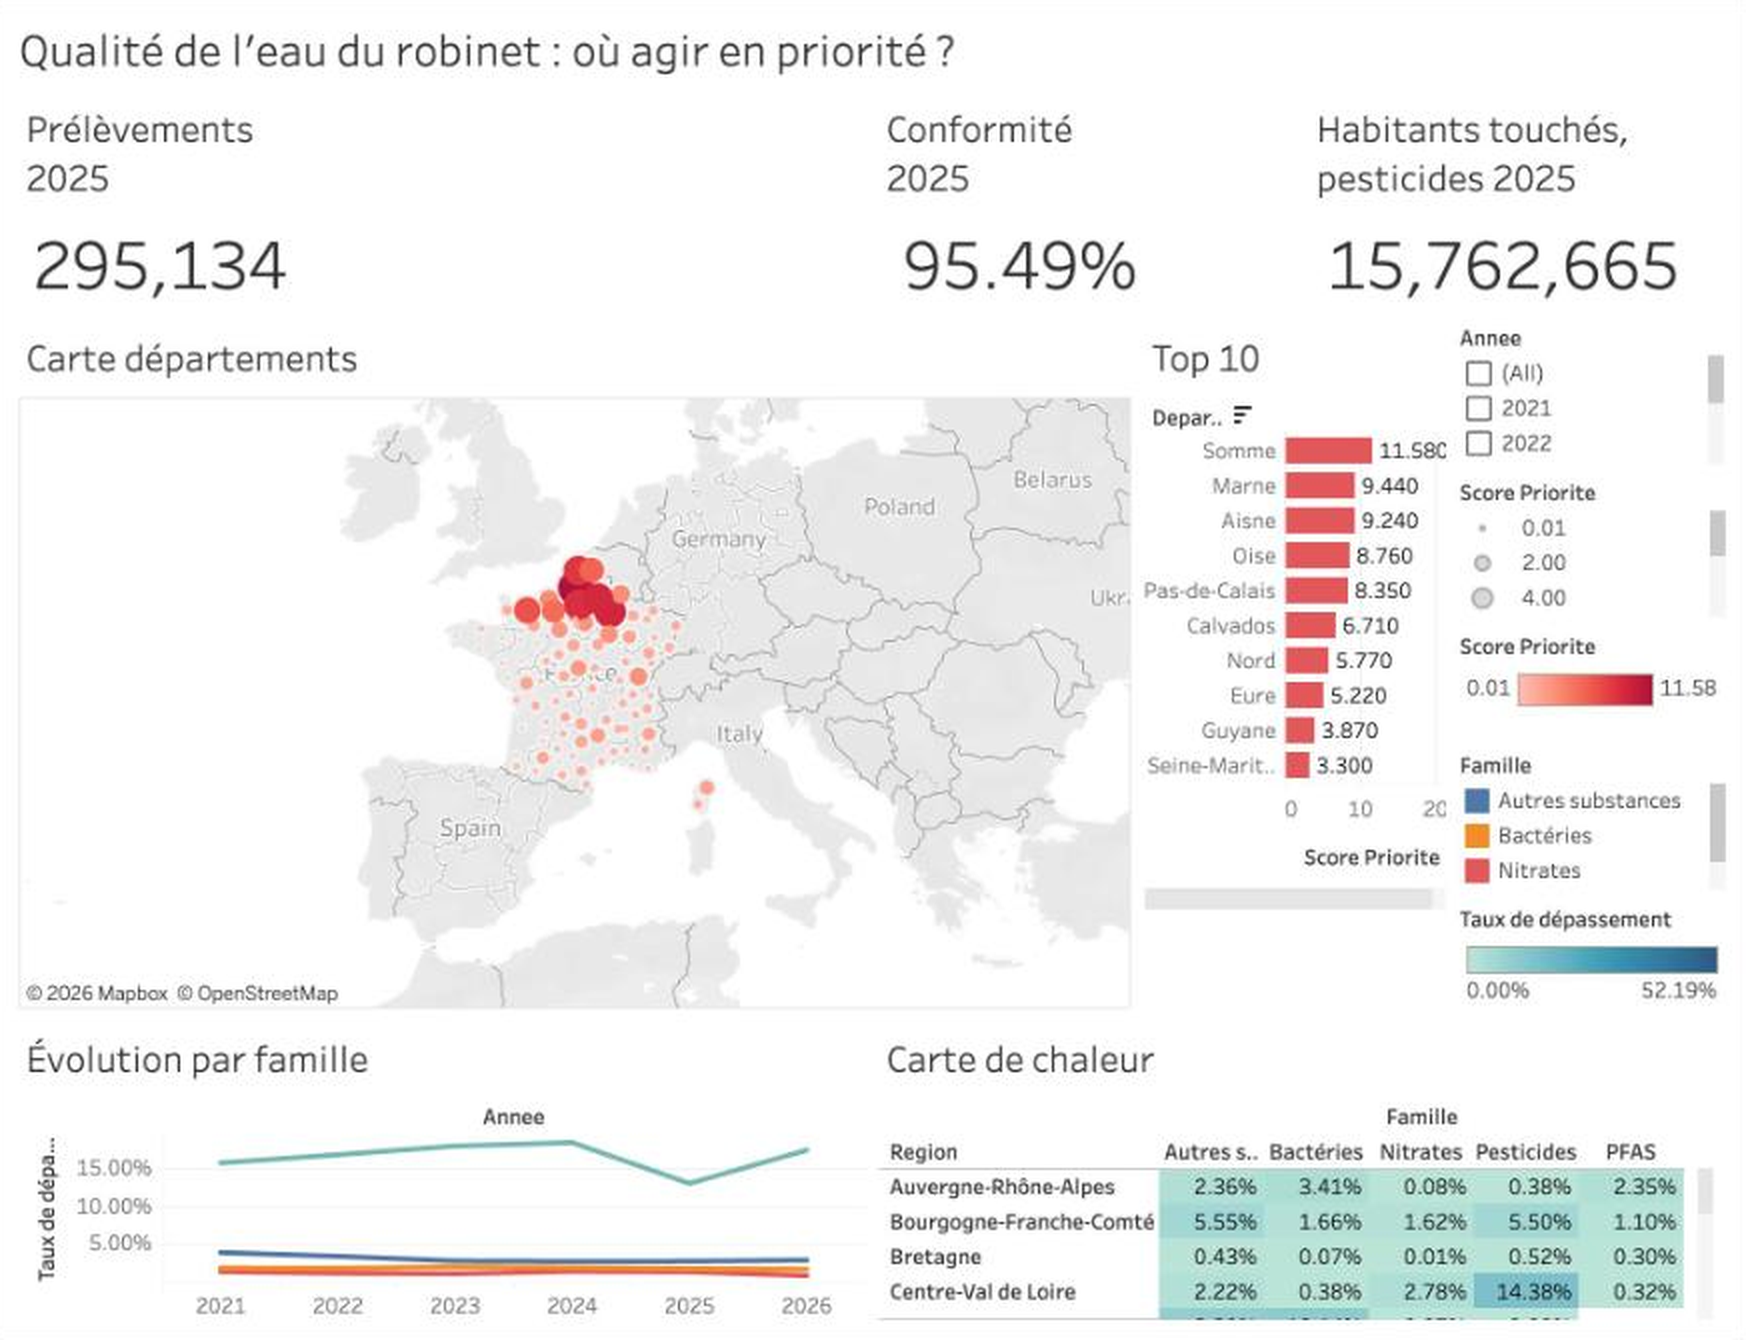
\includegraphics[width=0.85\textwidth]{vue_france.png}
\caption{Tableau de bord « Vue France »}
\label{fig:vuefrance}
\end{figure}

Le tableau de bord « Ma commune » (figure~\ref{fig:macommune}) s'adresse au citoyen. Il suffit de taper le nom de sa commune pour voir ses prélèvements, ses dépassements et son taux de dépassement par famille, ainsi que sa position sur la carte. Le département est ajouté au nom, car 3~660 communes partagent leur nom avec une autre. Le taux n'apparaît que si une seule commune est choisie. Un filtre permet de passer d'une famille de polluants à une autre. Lorsque le champ est vide, toute la France est affichée.

\begin{figure}[H]
\centering
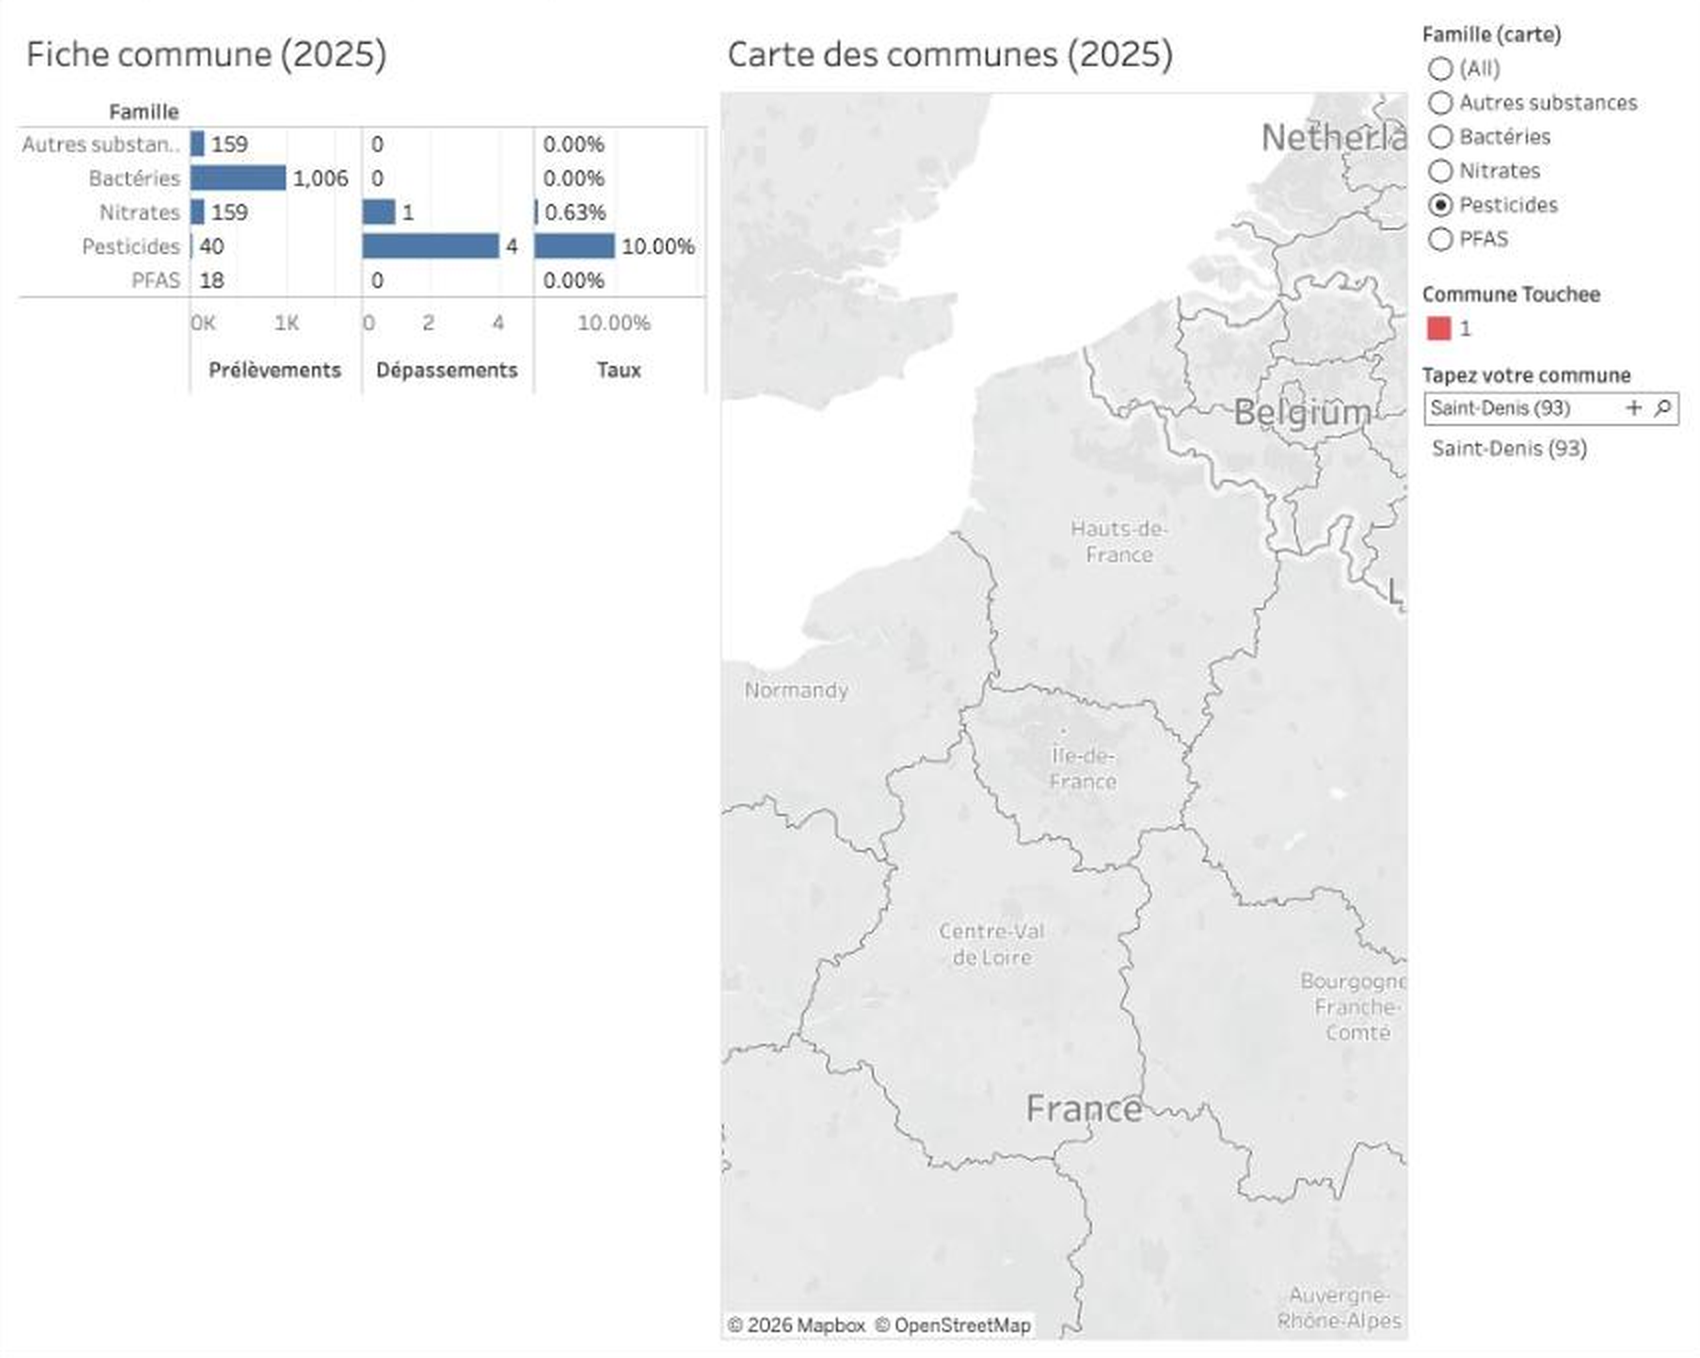
\includegraphics[width=0.75\textwidth]{ma_commune.png}
\caption{Tableau de bord « Ma commune »}
\label{fig:macommune}
\end{figure}

\subsection{Publication}

Le classeur a été publié sur Tableau Public, ce qui permet de le partager par un simple lien. Les données étant publiques, cette publication ne pose pas de problème de confidentialité. Le lien est donné en annexe.

% ------------------------------------------------------------------
\section{Résultats}
% ------------------------------------------------------------------

\subsection{Une eau globalement conforme}

Le premier résultat est plutôt rassurant : plus de 94~\% des prélèvements sont conformes chaque année (figure~\ref{fig:conformite}). La non-conformité augmente légèrement entre 2021 (5,45~\%) et 2024 (5,77~\%), puis passe à 4,51~\% en 2025, soit 95,5~\% de prélèvements conformes. Cette baisse ne doit pas être lue comme une amélioration équivalente de l'eau : en avril 2024, l'Anses a classé « non pertinent » le métabolite R471811 du chlorothalonil, qui n'a plus de limite de qualité dans nos données de 2025. En 2024, 2~727 prélèvements étaient non conformes uniquement à cause de lui. Sans eux, le taux de 2024 aurait été de 4,84~\%, donc environ les trois quarts de la baisse s'expliquent par ce changement. Les non-conformités chimiques sont près de deux fois plus fréquentes que les non-conformités bactériologiques : 8~742 contre 4~659 en 2025.

\begin{figure}[H]
\centering
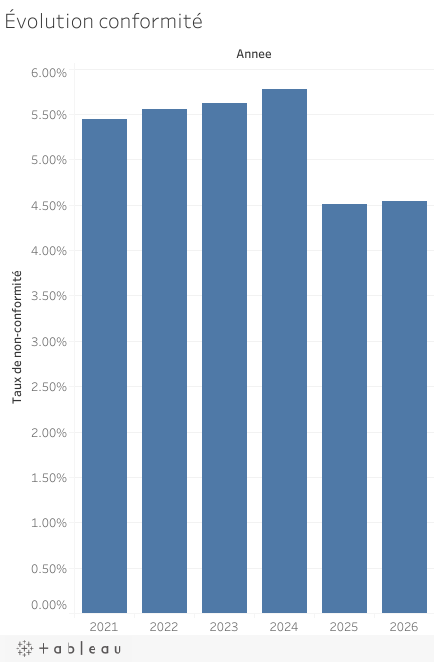
\includegraphics[width=0.4\textwidth]{evolution_conformite.png}
\caption{Taux de non-conformité des prélèvements par année}
\label{fig:conformite}
\end{figure}

\subsection{Les pesticides, premier problème}

La moyenne nationale cache cependant de fortes différences selon les familles et les territoires. Les pesticides sont de loin la famille qui dépasse le plus souvent : chaque année, entre 13 et 18,5~\% des prélèvements analysés pour les pesticides dépassent au moins une limite (tableau~\ref{tab:familles-evol} et figure~\ref{fig:famille}). Les autres familles restent sous 4~\%, et les bactéries et les nitrates autour de 1 à 2~\%.

\begin{table}[H]
\centering
\small
\begin{tabular}{lrrrrrr}
\toprule
Famille & 2021 & 2022 & 2023 & 2024 & 2025 & 2026 \\
\midrule
Pesticides & 15,8~\% & 16,9~\% & 18,0~\% & 18,5~\% & 13,1~\% & 17,5~\% \\
Autres substances & 3,9~\% & 3,4~\% & 2,8~\% & 2,7~\% & 2,7~\% & 2,9~\% \\
Bactéries & 1,8~\% & 1,8~\% & 2,0~\% & 1,9~\% & 1,7~\% & 1,7~\% \\
Nitrates & 1,3~\% & 1,1~\% & 1,1~\% & 1,4~\% & 1,3~\% & 0,8~\% \\
\bottomrule
\end{tabular}
\caption{Taux de dépassement par famille et par année (PFAS exclus)}
\label{tab:familles-evol}
\end{table}

\begin{figure}[H]
\centering
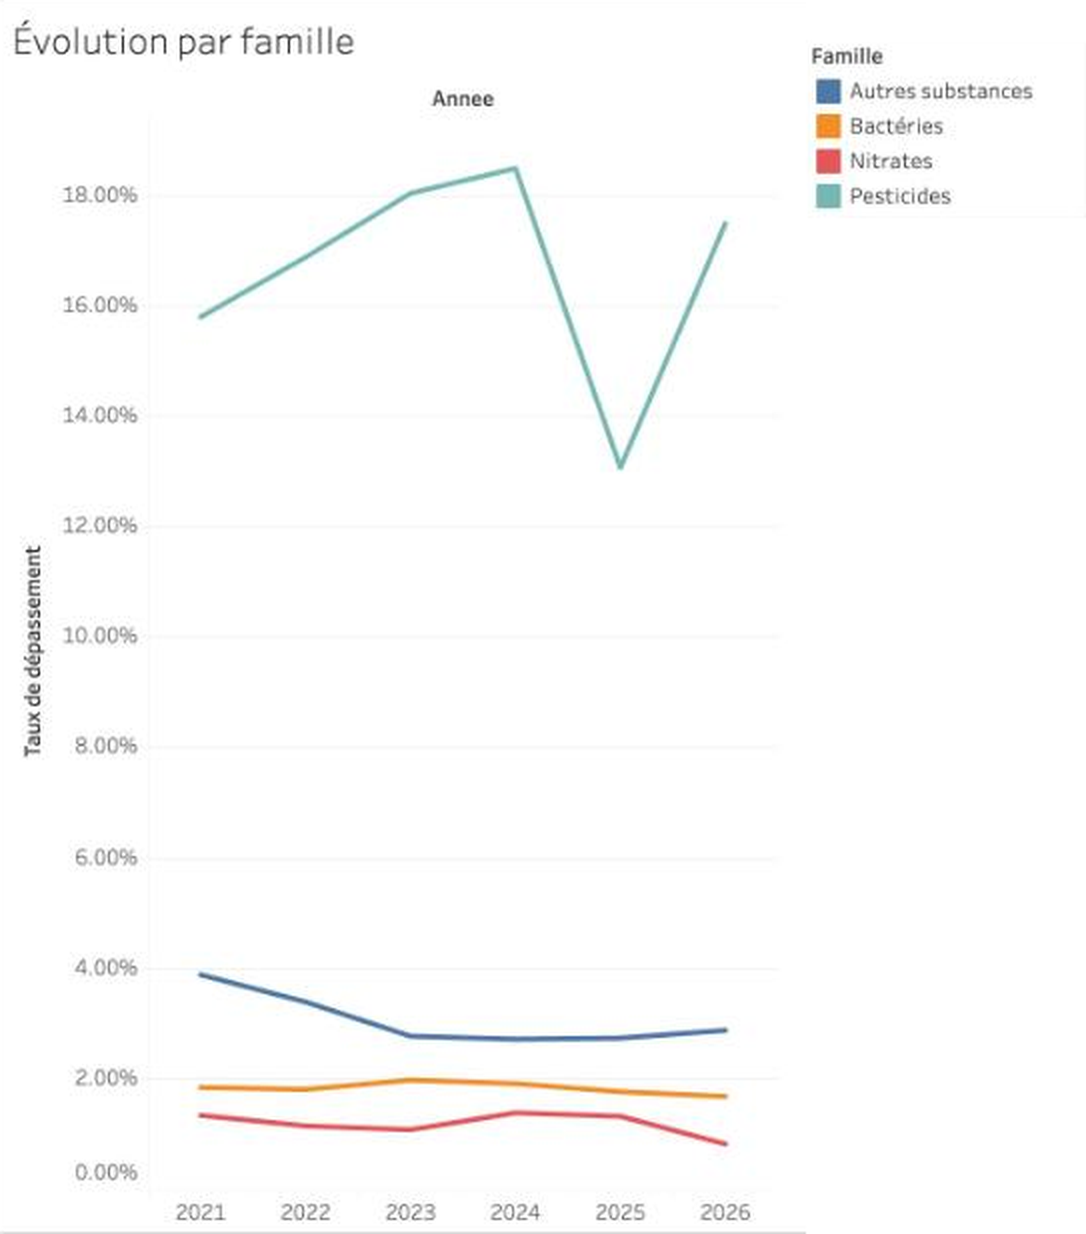
\includegraphics[width=0.6\textwidth]{evolution_famille.png}
\caption{Évolution du taux de dépassement par famille}
\label{fig:famille}
\end{figure}

La liste des molécules soumises à une limite change aussi d'une année à l'autre. Si l'on retire de toutes les années les deux principales molécules qui ont perdu leur limite (ESA métolachlore et R471811), le taux des pesticides est de 9,1~\% en 2021, 13,6~\% en 2023, 13,2~\% en 2024 et 13,1~\% en 2025. Il n'y a donc pas de baisse nette.

En 2025, 5~954 communes ont connu au moins un dépassement pour les pesticides. Elles comptent 15,8 millions d'habitants (tableau~\ref{tab:population}). La carte des communes (figure~\ref{fig:cartepest}) montre que ces communes se concentrent nettement dans le nord de la France : Hauts-de-France, Normandie et Grand Est. Cette répartition est cohérente avec l'origine agricole de ces substances, mais nos données ne permettent pas à elles seules de le démontrer.

\begin{table}[H]
\centering
\small
\begin{tabular}{lrr}
\toprule
Famille & Communes touchées & Population de ces communes \\
\midrule
Pesticides & 5~954 & 15~762~665 \\
Bactéries & 4~549 & 10~939~809 \\
Autres substances & 2~920 & 9~947~118 \\
Nitrates & 983 & 3~126~029 \\
PFAS & 172 & 926~954 \\
\bottomrule
\end{tabular}
\caption{Communes touchées et population concernée en 2025}
\label{tab:population}
\end{table}

\begin{figure}[H]
\centering
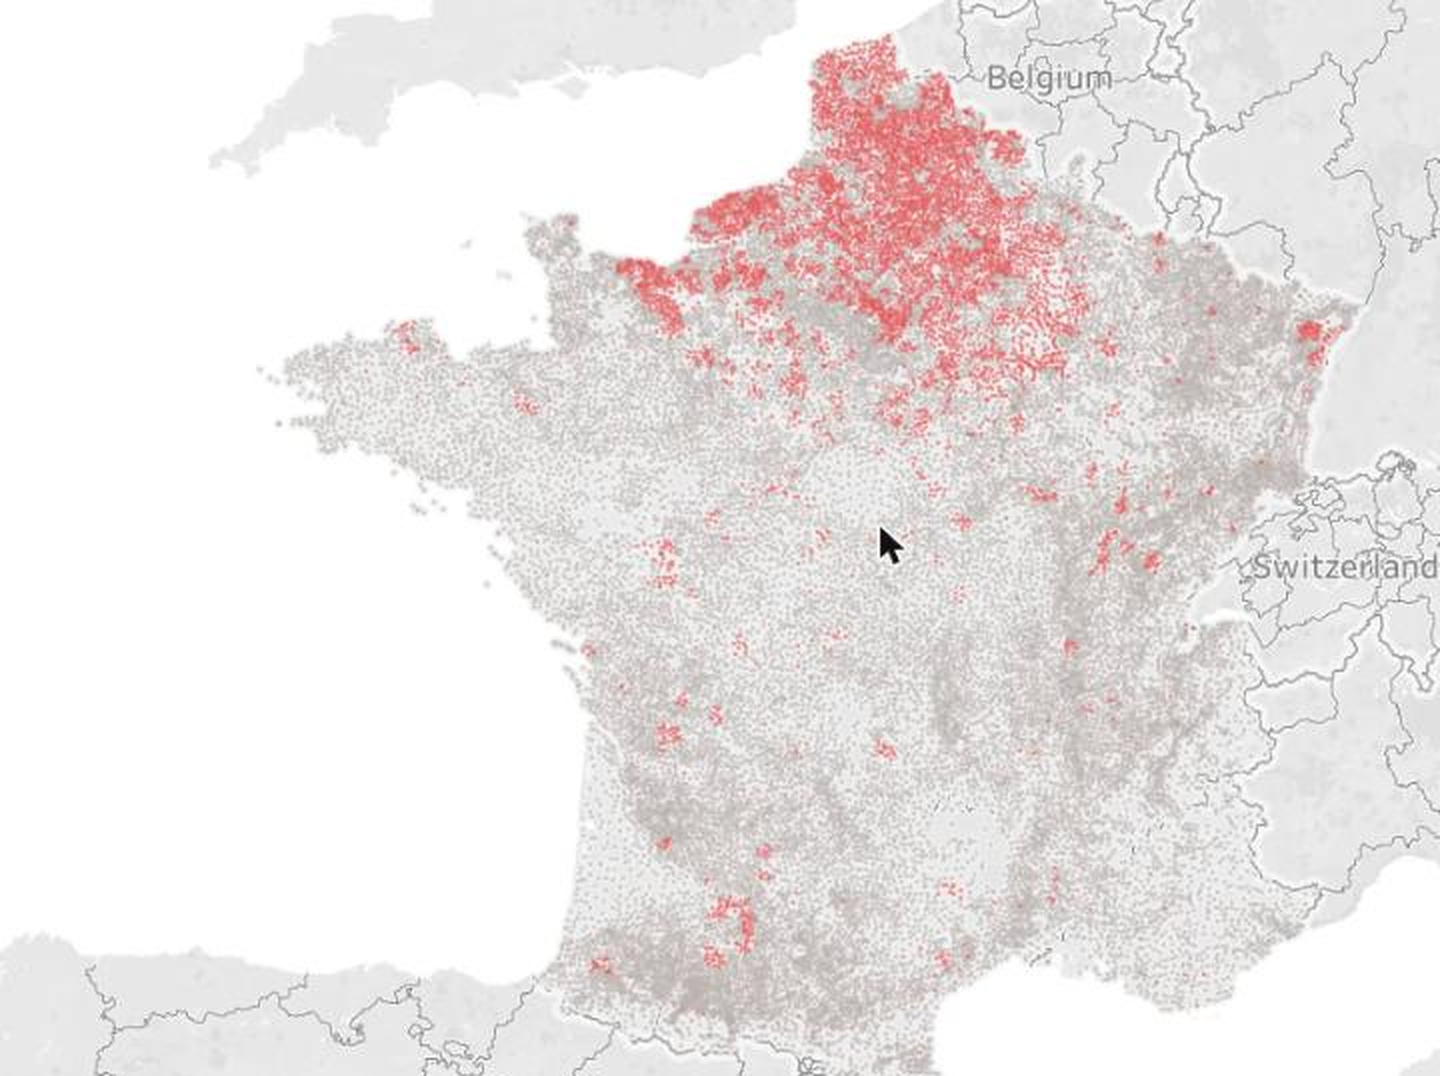
\includegraphics[width=0.75\textwidth]{carte_communes.png}
\caption{Communes avec au moins un dépassement pesticides en 2025, en rouge}
\label{fig:cartepest}
\end{figure}

\subsection{Une pollution en grande partie héritée}

Le classement des substances (figure~\ref{fig:substances}) montre que les dépassements de pesticides viennent surtout de métabolites, c'est-à-dire de produits de dégradation. La chloridazone desphényl arrive en tête avec 4~448 dépassements en 2025. Elle provient d'un herbicide utilisé surtout sur la betterave jusqu'à fin 2020. On retrouve aussi un métabolite du chlorothalonil, un fongicide utilisable en France jusqu'en mai 2020, et l'atrazine déséthyl, issue d'un herbicide du maïs interdit en 2003. Ces molécules persistent pendant des années dans les nappes : il s'agit donc en grande partie d'une pollution héritée du passé. Les bactéries \textit{E. coli} et entérocoques suivent, avec environ 3~000 dépassements chacune.

\begin{figure}[H]
\centering
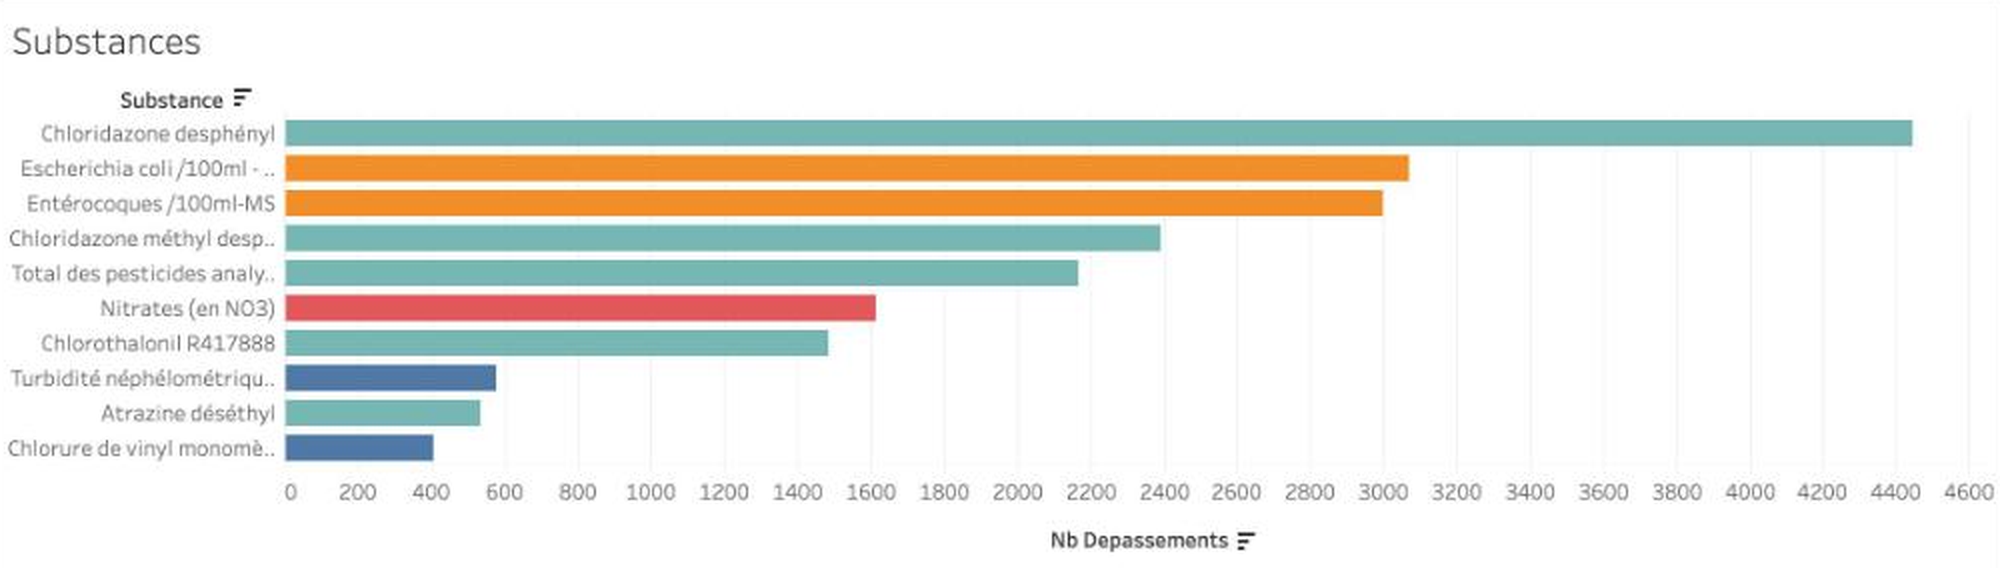
\includegraphics[width=0.95\textwidth]{substances.png}
\caption{Les dix substances avec le plus de dépassements en 2025}
\label{fig:substances}
\end{figure}

\subsection{Chaque région a son problème}

La carte de chaleur (figure~\ref{fig:chaleur}) croise les régions et les familles de polluants. Elle montre que les problèmes ne sont pas les mêmes partout. Les pesticides dominent dans le nord : un peu plus d'un prélèvement analysé sur deux est en dépassement en Hauts-de-France (52,2~\%), contre 27,3~\% en Normandie et 21,6~\% dans le Grand Est. Les bactéries posent surtout problème en Corse (10,1~\%) et en Guyane (5,6~\%). Au niveau des communes, le taux est de 0,83~\% dans celles de moins de 2~000 habitants, contre 0,10~\% au-delà de 10~000. La famille « autres substances » est très présente en Guyane (25,4~\%), surtout à cause de la turbidité et des trihalométhanes.

\begin{figure}[H]
\centering
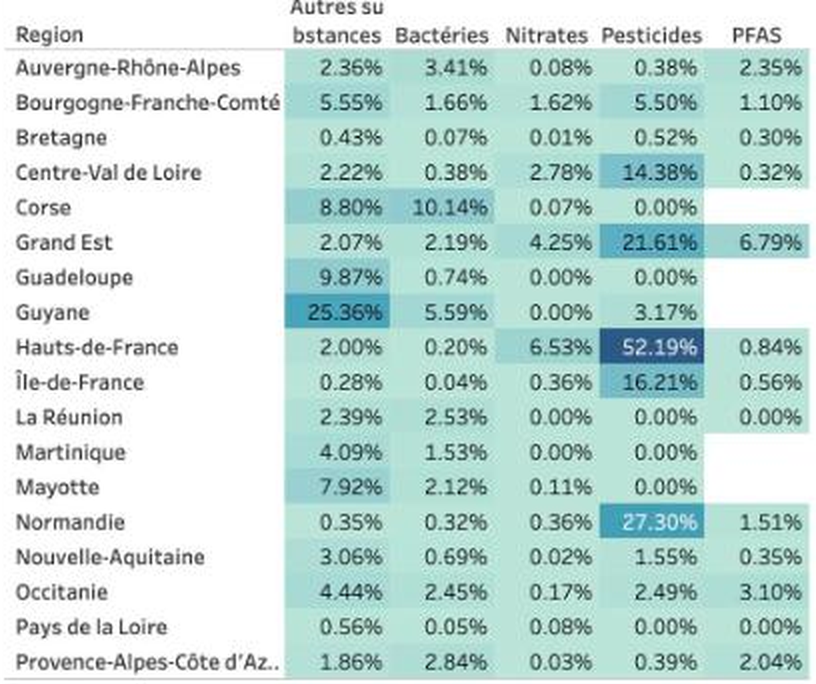
\includegraphics[width=0.7\textwidth]{carte_chaleur.png}
\caption{Taux de dépassement par région et par famille en 2025 (case vide : non mesuré)}
\label{fig:chaleur}
\end{figure}

\subsection{Les PFAS, un enjeu émergent}

Avec la nouvelle limite européenne de 0,1~µg/L pour la somme de 20 PFAS, 172 communes ont eu en 2025 au moins une mesure au-dessus de ce seuil, que nous avons appliqué à toutes les années, pour une population d'environ 927~000 habitants. Les plus grandes sont Besançon, Cherbourg-en-Cotentin (jusqu'à 4,6 fois la limite), Chambéry et Narbonne. Les premiers signaux apparaissent surtout dans le Grand Est (6,8~\% de dépassement), en Occitanie (3,1~\%) et en Auvergne-Rhône-Alpes (2,3~\%). Ces mesures étant récentes, la situation devra être suivie dans les prochaines années.

\subsection{Les départements prioritaires}

Le score de priorité permet enfin de répondre directement à notre problématique (tableau~\ref{tab:top10} et figure~\ref{fig:top10}). La Somme arrive en tête avec un score de 11,58, devant la Marne et l'Aisne. Cinq des dix premiers départements sont en Hauts-de-France et trois en Normandie. Le score est surtout porté par les pesticides. La Guyane fait figure d'exception : elle apparaît dans le classement à cause des bactéries et des autres substances.

\begin{table}[H]
\centering
\small
\begin{tabular}{clll}
\toprule
Rang & Département & Région & Score \\
\midrule
1 & Somme & Hauts-de-France & 11,58 \\
2 & Marne & Grand Est & 9,44 \\
3 & Aisne & Hauts-de-France & 9,24 \\
4 & Oise & Hauts-de-France & 8,76 \\
5 & Pas-de-Calais & Hauts-de-France & 8,35 \\
6 & Calvados & Normandie & 6,71 \\
7 & Nord & Hauts-de-France & 5,77 \\
8 & Eure & Normandie & 5,22 \\
9 & Guyane & Guyane & 3,87 \\
10 & Seine-Maritime & Normandie & 3,30 \\
\bottomrule
\end{tabular}
\caption{Les dix départements prioritaires en 2025}
\label{tab:top10}
\end{table}

\begin{figure}[H]
\centering
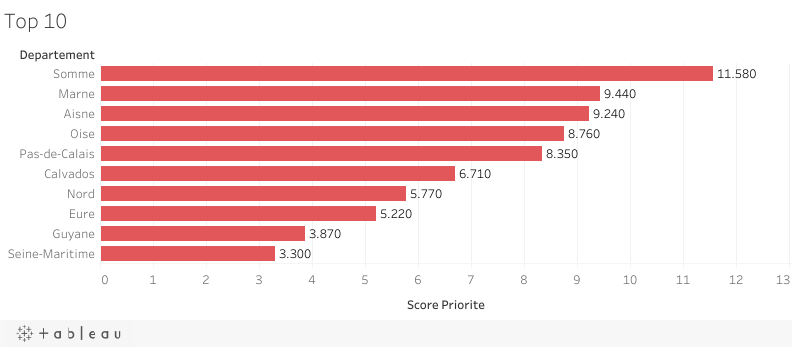
\includegraphics[width=0.75\textwidth]{top10.png}
\caption{Top 10 des départements selon le score de priorité (2025)}
\label{fig:top10}
\end{figure}

% ------------------------------------------------------------------
\section{Aide à la décision}
% ------------------------------------------------------------------

\subsection{Ce qu'il faut retenir}

Nos résultats peuvent se résumer en cinq points. L'eau du robinet est globalement de bonne qualité, avec 95,5~\% de prélèvements conformes en 2025. Les pesticides restent pourtant le premier problème : 5~954 communes et 15,8 millions d'habitants sont concernés. Ce problème est très concentré dans le nord de la France. Les substances les plus souvent en cause viennent en grande partie de molécules interdites depuis plusieurs années. Enfin, les PFAS apparaissent comme le prochain enjeu, avec 172 communes au-dessus de la nouvelle limite.

\subsection{Recommandations pour une ARS}

À partir de ces résultats, nous proposons les actions suivantes (tableau~\ref{tab:reco}).

\begin{table}[H]
\centering
\small
\begin{tabular}{c >{\raggedright}p{7.2cm} >{\raggedright\arraybackslash}p{5.6cm}}
\toprule
Priorité & Action & Territoires \\
\midrule
1 & Traiter les métabolites de pesticides (filtration sur charbon actif, interconnexion de réseaux, dilution) & Somme, Marne, Aisne, Oise, Pas-de-Calais \\
2 & Protéger les captages (aires d'alimentation, réduction des intrants agricoles) & Hauts-de-France, Normandie, Grand Est \\
3 & Renforcer la surveillance des PFAS et informer la population & Grand Est, Occitanie, Auvergne-Rhône-Alpes \\
4 & Améliorer le traitement bactériologique des petits réseaux & Corse, Guyane, petites communes \\
5 & Informer les citoyens avec l'outil « Ma commune » & Toute la France \\
\bottomrule
\end{tabular}
\caption{Recommandations proposées}
\label{tab:reco}
\end{table}

\subsection{Apport de la visualisation}

Sans visualisation, ces informations sont enfermées dans plus de 11~Go de fichiers difficilement lisibles. Avec les tableaux de bord, un décideur peut voir en quelques secondes où se trouvent les problèmes et quels départements traiter en premier, puis approfondir en cliquant sur un territoire. Pour le citoyen, l'outil « Ma commune » donne une réponse simple à une question qui le concerne directement.

% ------------------------------------------------------------------
\section{Limites}
% ------------------------------------------------------------------

Notre travail comporte plusieurs limites qu'il faut garder en tête pour interpréter les résultats.

\begin{itemize}
  \item \textbf{Le choix des poids.} Le score de priorité dépend des poids retenus. D'autres pondérations donneraient un classement différent, en particulier le poids de 10~\% donné aux autres substances, qui comprennent aussi des métaux comme le plomb et l'arsenic.
  \item \textbf{La couverture des PFAS.} Les PFAS étaient très peu mesurés avant 2025. Leur évolution dans le temps ne peut donc pas être interprétée.
  \item \textbf{L'année 2026.} Les données de 2026 s'arrêtent au 30~septembre et sont donc incomplètes.
  \item \textbf{Dépassement et danger.} Une limite de qualité est une valeur de précaution. Un dépassement ne signifie pas forcément un danger immédiat, et c'est l'ARS qui évalue ensuite le risque et décide d'éventuelles restrictions.
  \item \textbf{La notion de commune touchée.} Une commune est comptée comme touchée dès un seul dépassement dans l'année, et toute sa population est comptée même si une partie seulement du réseau est concernée. La population exposée est donc un majorant.
  \item \textbf{Les changements de réglementation.} Plusieurs métabolites ont perdu leur limite de qualité entre 2021 et 2025. Les taux de plusieurs années ne sont donc pas strictement comparables.
  \item \textbf{Les données manquantes.} Une famille non mesurée compte pour zéro dans le score, qui peut donc être sous-estimé.
  \item \textbf{Le classement des pesticides.} Il repose sur la valeur de la limite réglementaire et non sur une liste vérifiée molécule par molécule.
\end{itemize}

% ------------------------------------------------------------------
\section{Conclusion}
% ------------------------------------------------------------------

Ce projet nous a permis de passer de fichiers bruts très volumineux à deux tableaux de bord utilisables par un décideur et par un citoyen. Il répond à notre problématique : l'eau du robinet est conforme à plus de 95~\% en 2025, mais 15,8 millions de personnes vivent dans une commune touchée par les pesticides, surtout dans le nord de la France. C'est là qu'une ARS devrait agir en priorité, en commençant par la Somme, la Marne et l'Aisne.

Sur le plan technique, le projet nous a fait travailler la préparation de données volumineuses, le choix d'indicateurs comparables et plusieurs fonctionnalités de Tableau : cartes, calculs de table, expressions de niveau de détail, filtres de contexte et actions de filtre.

Pour aller plus loin, il serait intéressant de suivre l'évolution des PFAS dans les années à venir, maintenant que les mesures sont généralisées, et de croiser ces résultats avec d'autres données, comme les surfaces agricoles ou la localisation des sites industriels.

\appendix

% ------------------------------------------------------------------
\section{Formules des champs calculés}
% ------------------------------------------------------------------

\small
\begin{longtable}{>{\raggedright}p{4cm} >{\raggedright\arraybackslash}p{10cm}}
\toprule
Champ & Formule Tableau \\
\midrule
\endhead
Taux de dépassement & \texttt{SUM([nb\_prelevements\_depassement\_communes]) / SUM([nb\_prelevements\_communes])} \\
Part de la population exposée & \texttt{SUM([population\_exposee]) / SUM([population\_controlee])} \\
Taux de non-conformité & \texttt{SUM([nb\_non\_conformes]) / SUM([nb\_prelevements])} \\
Taux de conformité & \texttt{1 - [Taux de non-conformité]} \\
Variation sur un an & \texttt{(SUM([nb\_non\_conformes]) / SUM([nb\_prelevements])) - LOOKUP(SUM([nb\_non\_conformes]) / SUM([nb\_prelevements]), -1)} \\
Score recalculé & \texttt{0.30*ZN([risque\_bacteries\_pct]) + 0.20*ZN([risque\_nitrates\_pct]) + 0.20*ZN([risque\_pesticides\_pct]) + 0.20*ZN([risque\_pfas\_pct]) + 0.10*ZN([risque\_autres\_pct])} \\
Rang du département & \texttt{RANK(SUM([score\_priorite]))} \\
Population de la région & \texttt{\{ FIXED [region], [annee] : SUM([population\_dept]) \}} \\
Population de la commune & \texttt{\{ FIXED [code\_insee] : MAX([population]) \}} \\
Population exposée & \texttt{IF [commune\_touchee] = 1 THEN [population] END} \\
Taux (fiche commune) & \texttt{IF COUNTD([Code Insee]) = 1 THEN SUM([Nb Prelevements Depassement]) / SUM([Nb Prelevements]) END} \\
\bottomrule
\end{longtable}
\normalsize

% ------------------------------------------------------------------
\section{Glossaire}
% ------------------------------------------------------------------

\begin{description}
  \item[ARS] Agence régionale de santé, chargée d'organiser le contrôle sanitaire de l'eau.
  \item[Contrôle sanitaire] Programme officiel de prélèvements et d'analyses de l'eau distribuée.
  \item[Limite de qualité] Valeur réglementaire à ne pas dépasser pour un paramètre.
  \item[Métabolite] Produit de dégradation d'un pesticide dans l'environnement.
  \item[PFAS] Substances per- et polyfluoroalkylées, dites « polluants éternels ».
  \item[Calcul de table] Calcul effectué sur les résultats affichés dans une vue (RANK, LOOKUP).
  \item[Expression LOD] Calcul réalisé à un niveau de détail fixé, indépendamment de l'affichage (FIXED).
  \item[Filtre de contexte] Filtre appliqué avant les autres filtres, notamment avant un Top N.
  \item[Action de filtre] Clic sur un graphique qui filtre les autres graphiques d'un tableau de bord.
\end{description}

% ------------------------------------------------------------------
\section{Sources et liens}
% ------------------------------------------------------------------

\begin{itemize}
  \item Ministère de la Santé, « Résultats du contrôle sanitaire de l'eau distribuée commune par commune », data.gouv.fr, fichiers 2021 à 2026, Licence Ouverte.
  \item Ministère de la Santé, documentation du jeu de données (description des fichiers, version 7, 2021).
  \item Insee, référentiel des communes (population et coordonnées), via geo.api.gouv.fr.
  \item ARS Hauts-de-France, « Les métabolites du chlorothalonil » et « Recherche des métabolites de la chloridazone dans l'eau du robinet ».
  \item ARS Bourgogne-Franche-Comté, note sur le classement du R471811 (avis de l'Anses du 29 avril 2024).
  \item Banque des Territoires, « L'eau potable largement contaminée par des résidus d'un fongicide interdit ».
  \item Assemblée nationale, réponses ministérielles sur l'interdiction de l'atrazine (2003-2004).
  \item Classeur Tableau Public du projet :\\ \url{https://public.tableau.com/app/profile/mohammed.benakka.ouayad/viz/Qualitdeleaudurobinet/VueFrance}
\end{itemize}

\end{document}
